\section{Diagrammi}

\begin{center}
	\begin{tikzpicture}[scale=0.65]
		\pie[color = {red!70, yellow!70, green!70, cyan!70}] {
			20/Rosso,
			25/Giallo,
			30/Verde,
			25/Blu
		}
	\end{tikzpicture}
\end{center}

\begin{center}
	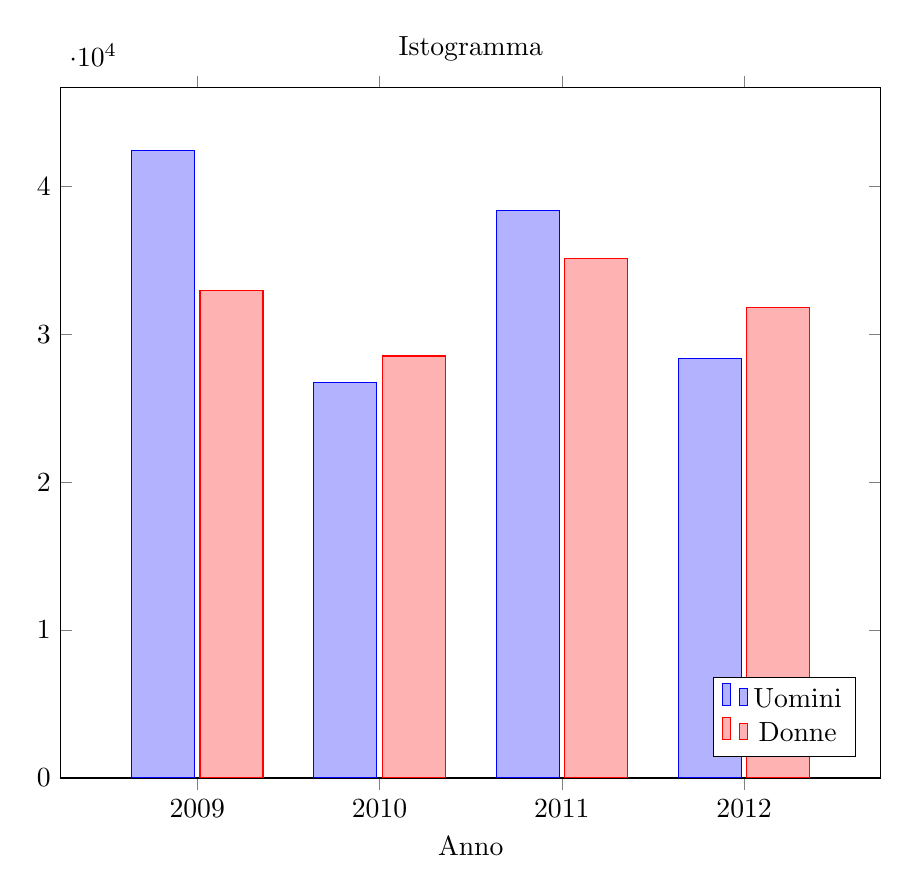
\begin{tikzpicture}
		\begin{axis}[
				title={Istogramma},
				width=12cm,
				x tick label style={/pgf/number format/1000 sep={}},
				xlabel={Anno},
				xtick = {2009, 2010, 2011, 2012},
				ytick = {0, 10000, 20000, 30000, 40000, 50000},
				enlarge x limits=0.25,
				ybar,
				bar width=0.8cm,
				ymin=0,
				legend style={legend columns=1},
				legend pos=south east
			]

			\addplot coordinates { (2009, 42433) (2010, 26756) (2011, 38381) (2012, 28349) };

			\addplot coordinates { (2009, 32957) (2010, 28532) (2011, 35124) (2012, 31828) };

			\legend{Uomini, Donne}
		\end{axis}
	\end{tikzpicture}
\end{center}
